\documentclass[12pt]{article}
\usepackage[english]{babel}
\usepackage[utf8x]{inputenc}
\usepackage[T1]{fontenc}
\usepackage{lab}
\usepackage{listings}
\usepackage{comment}


\Instructors{Alex Mussa, Kevin Johnson}
\LabNumber{3}
\LabTitle{Circuit Prototyping and Testing}
\LabDate{July 1st, 2019}

\lstset{style=mystyle}

\begin{document}
\MakeLabTop

\section{Introduction}

In these lab experiments, fundamental circuit elements in the use of controlling and interfacing with circuits such as switches and potentiometers, and dc motors will be explored. These devices effectively allow a user to send a signal at a desired time to a device such as a circuit or a microcontroller to notify it something should occur. These signals can take many forms, such as DC or various AC waveforms. These signals can be utilized for making decisions such as when to turn on the motors to move a robot and also how fast the motor should go. 

These control mechanisms depend greatly on the shape or behavior of the waveform used to do the controlling. The waveforms physical changing of behavior of an LED, for example, can be visualized by applying various waveform. Some waves, such as the square wave, are used to control a motors behavior in pulse width modulation. 

\section{Setup}

\subsection{Collecting Materials}

First, collect the following items from the Tumbller robot's kit:

\begin{enumerate}
    \item 2 3.7V Rechargeable Batteries
    \item Battery Charger
\end{enumerate}

\begin{figure}[H]
    \centering
    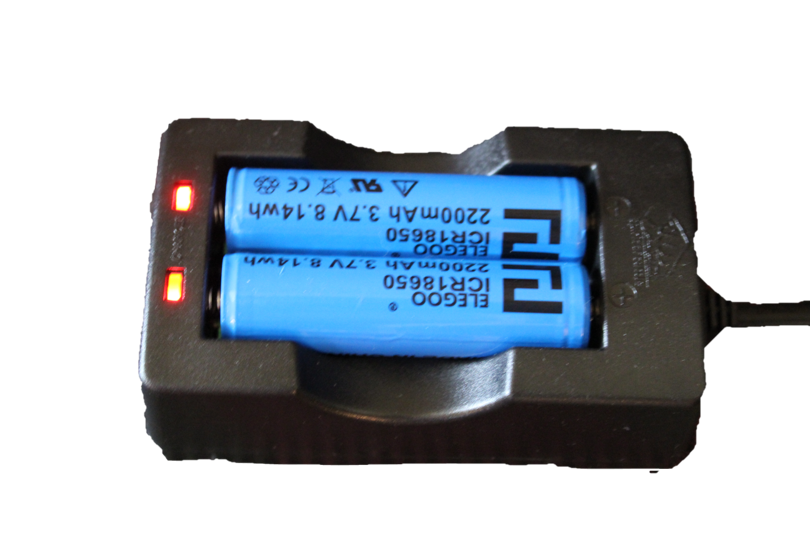
\includegraphics[width=6cm]{photos/lab/batteriescharger.png}
    \caption{Batteries and charger.}
\end{figure}

Once you have found these, put the batteries in the charger and plug it into a power outlet at the lab bench. Place the unit to the side and let it charge. Continue gather the following from the Tumbller robot's kit:

\begin{enumerate}
    \item Battery housing with switch
    \item TB6122FGN Motor Controller (Red 16 Pin PCB)
    \item 1 DC Motor
    \item 1 DC Motor connection cable (6-pin)
\end{enumerate}

\begin{figure}[H]
\begin{subfigure}{.5\textwidth}
    \centering
    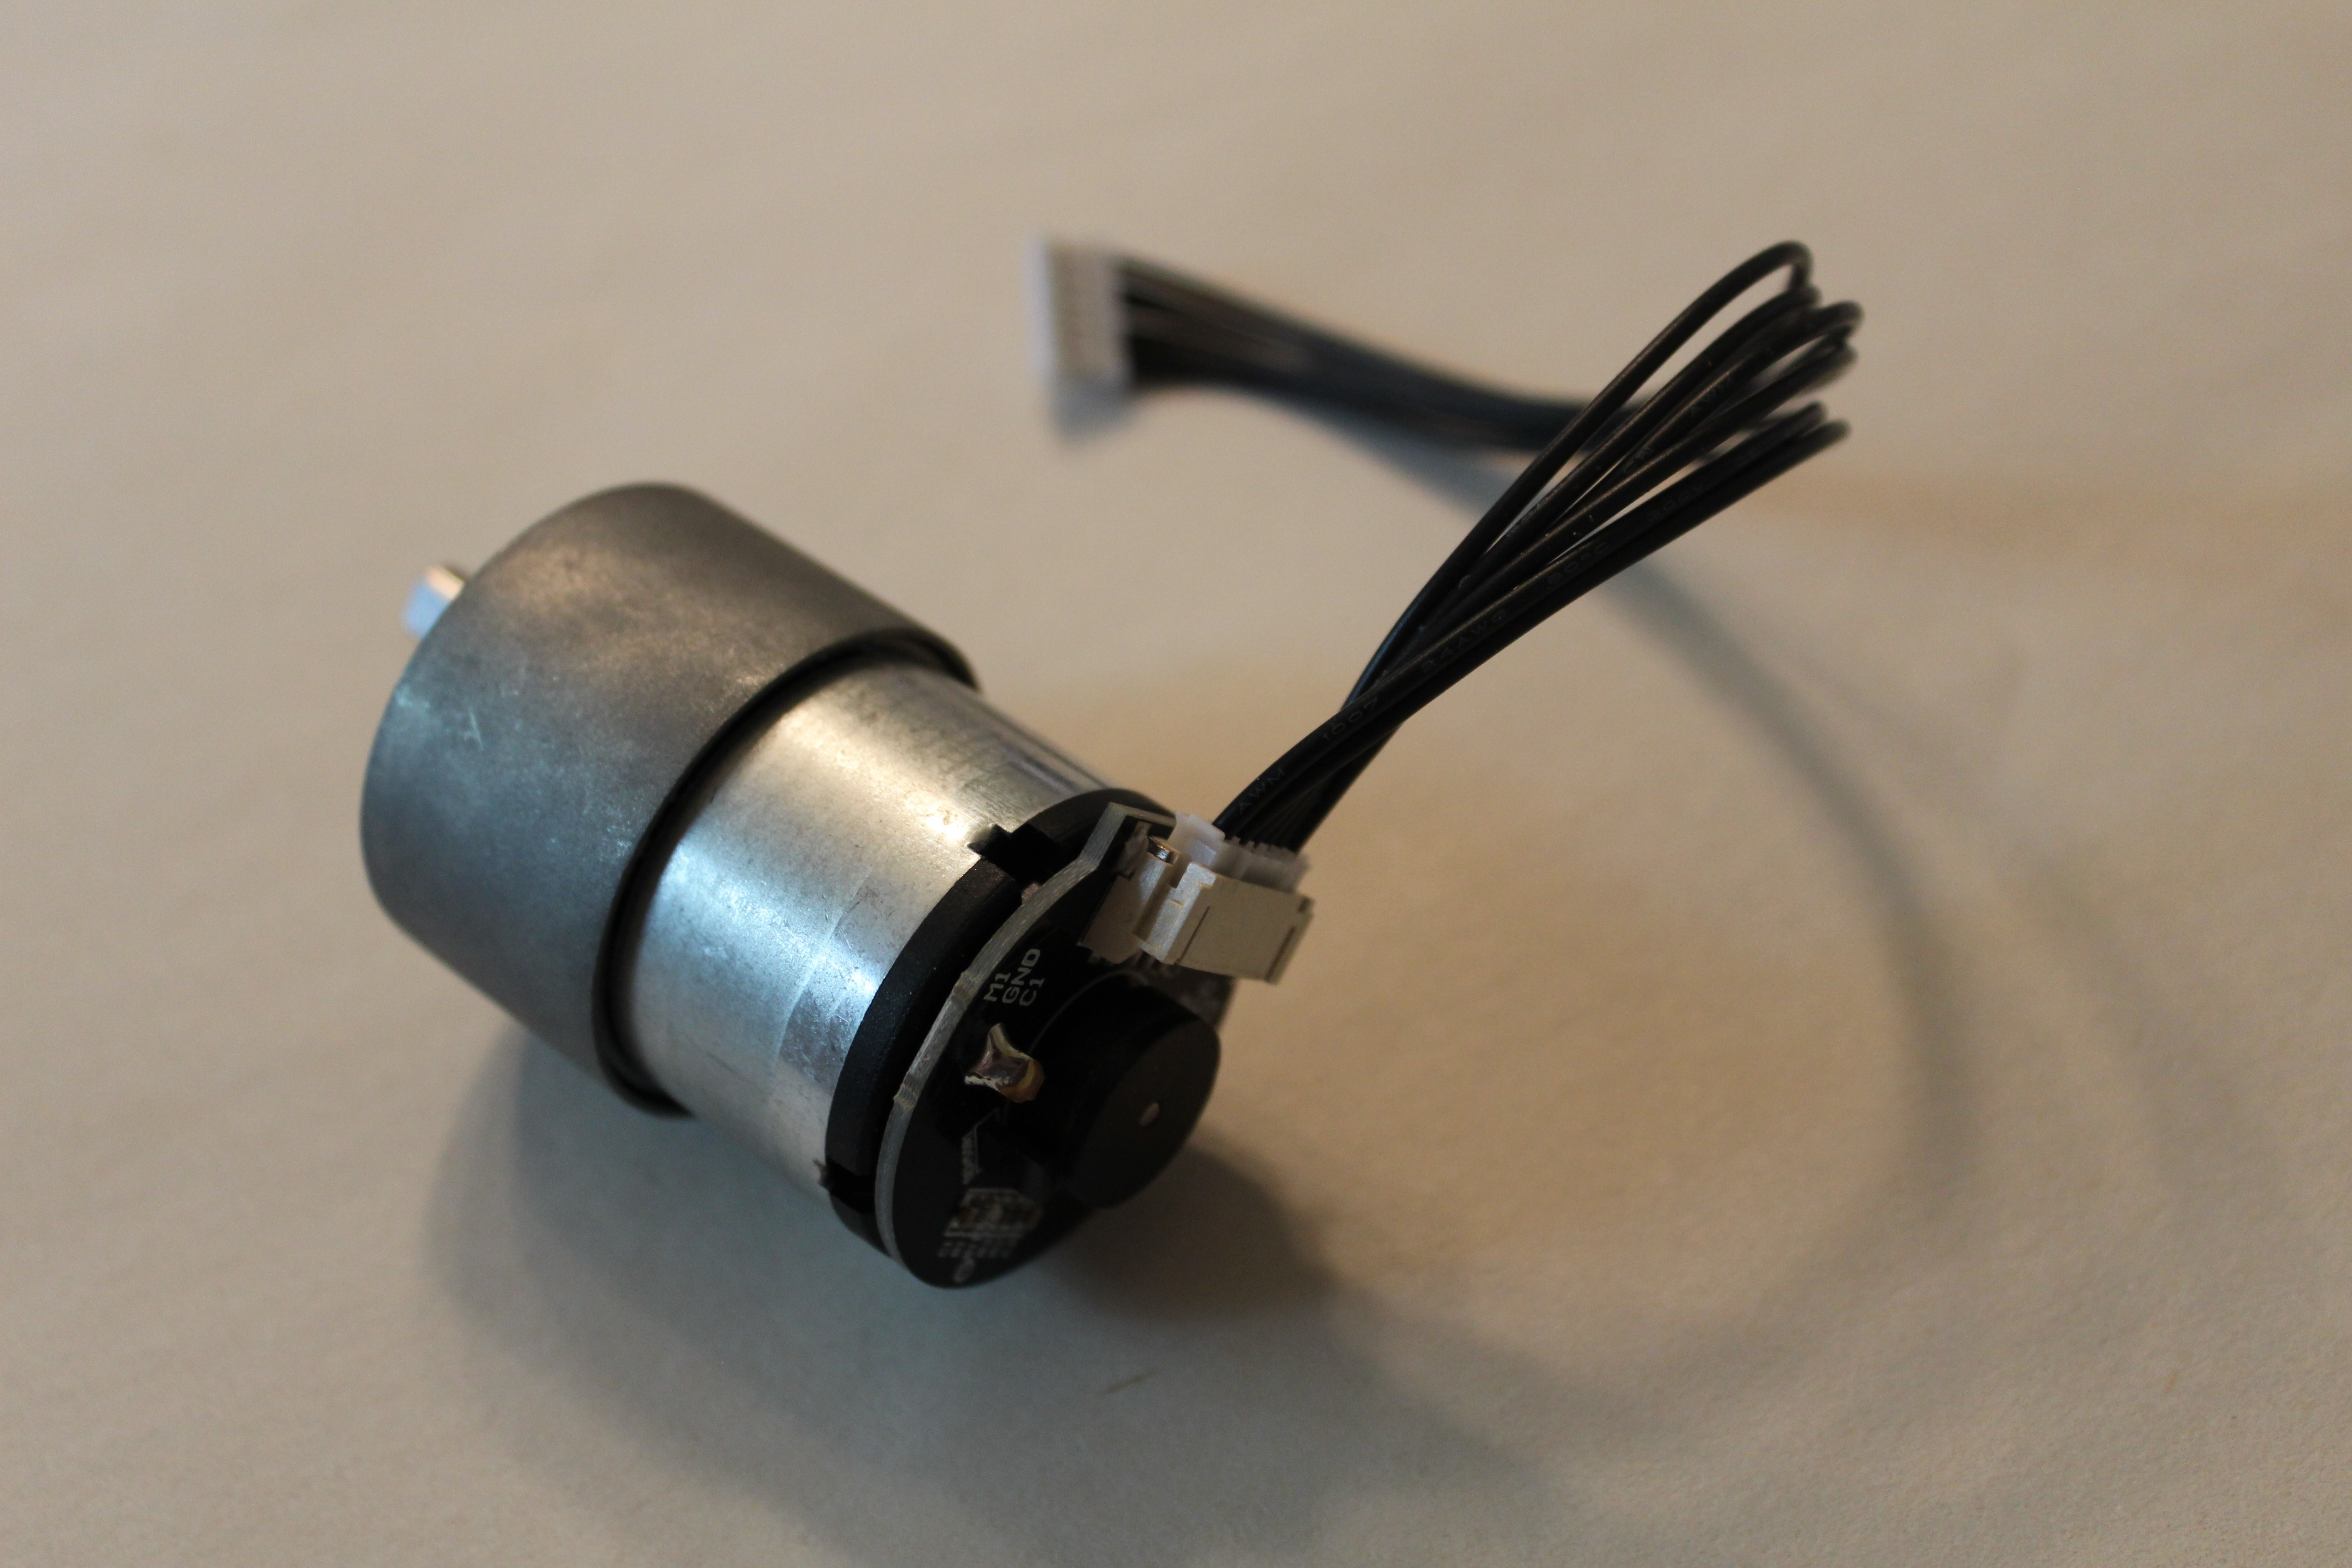
\includegraphics[width=0.8\linewidth]{photos/lab/motor.jpg}
    \caption{DC Motor with cable.}
\end{subfigure}%
\begin{subfigure}{.5\textwidth}
  \centering
  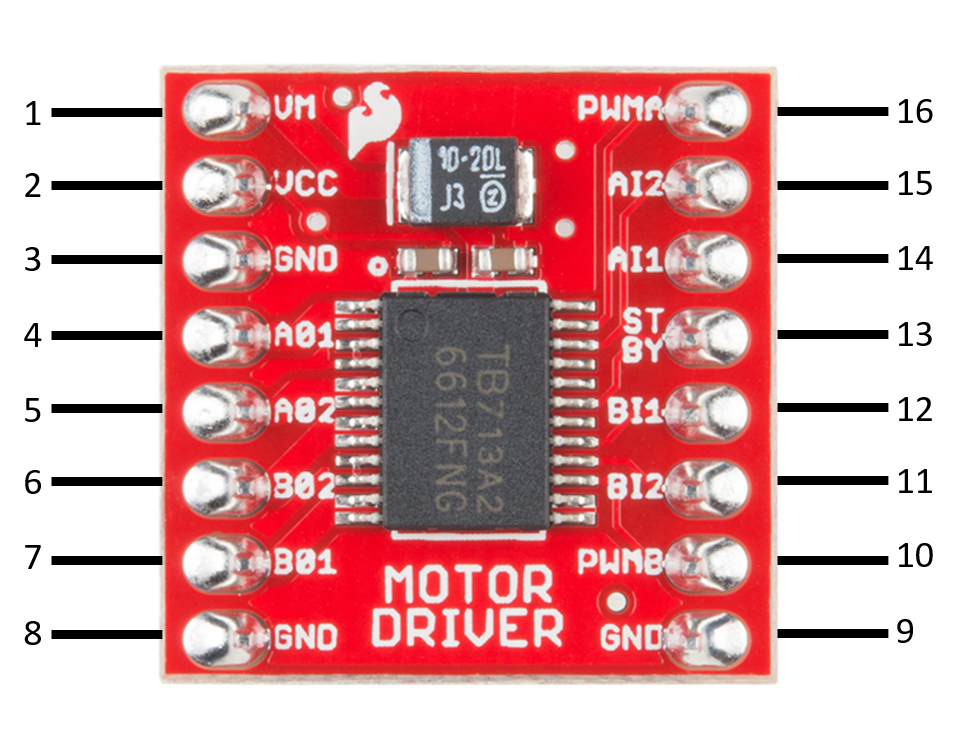
\includegraphics[width=0.79\linewidth]{photos/lab/motordriver.png}
  \caption{TB6122FGN Motor Controller}
\end{subfigure}
\caption{Top and bottom view of a potentiometer.}
\end{figure}

Then, collect the push button sensor from the 37 Sensor kit. 

Next, collect the following items from the instructors:

\begin{itemize}
    \item Breadboard
    \item Wires
    \item LED
    \item Potentiometer
\end{itemize}

When you have all of the above items, continue on to perform the experiments below.

\section{Experiments}
\subsection{Controlling an LEDs brightness}

In the previous lab exercises, the LED and some of its basic properties were explored such as turn on voltage. It was noticed that as the voltage value applied across the LEDs anode and cathode increased from zero that initially the LED did not turn on. After a voltage value, called the turn on voltage, the LED began getting brighter and brighter. With this basic knowledge of how LEDS behave at different voltage levels, AC signals can be utilized to take advantage of this as time elapses.

The DC power supply being used to illuminate the LED previously stays at the same voltage value as time elapses. That means the LEDs brightness does not change as time ellapses. However, the potentiometer can be utilized to vary the voltage applied to the LED and control the brightness manually. This ability to vary a voltage to a precise desired value can be utilized outside of controlling an LEDs brightness in applications such as setting an amplifiers volume, selecting setting values for , and communicating setting with a microcontroller.

\begin{figure}[H]
    \centering
    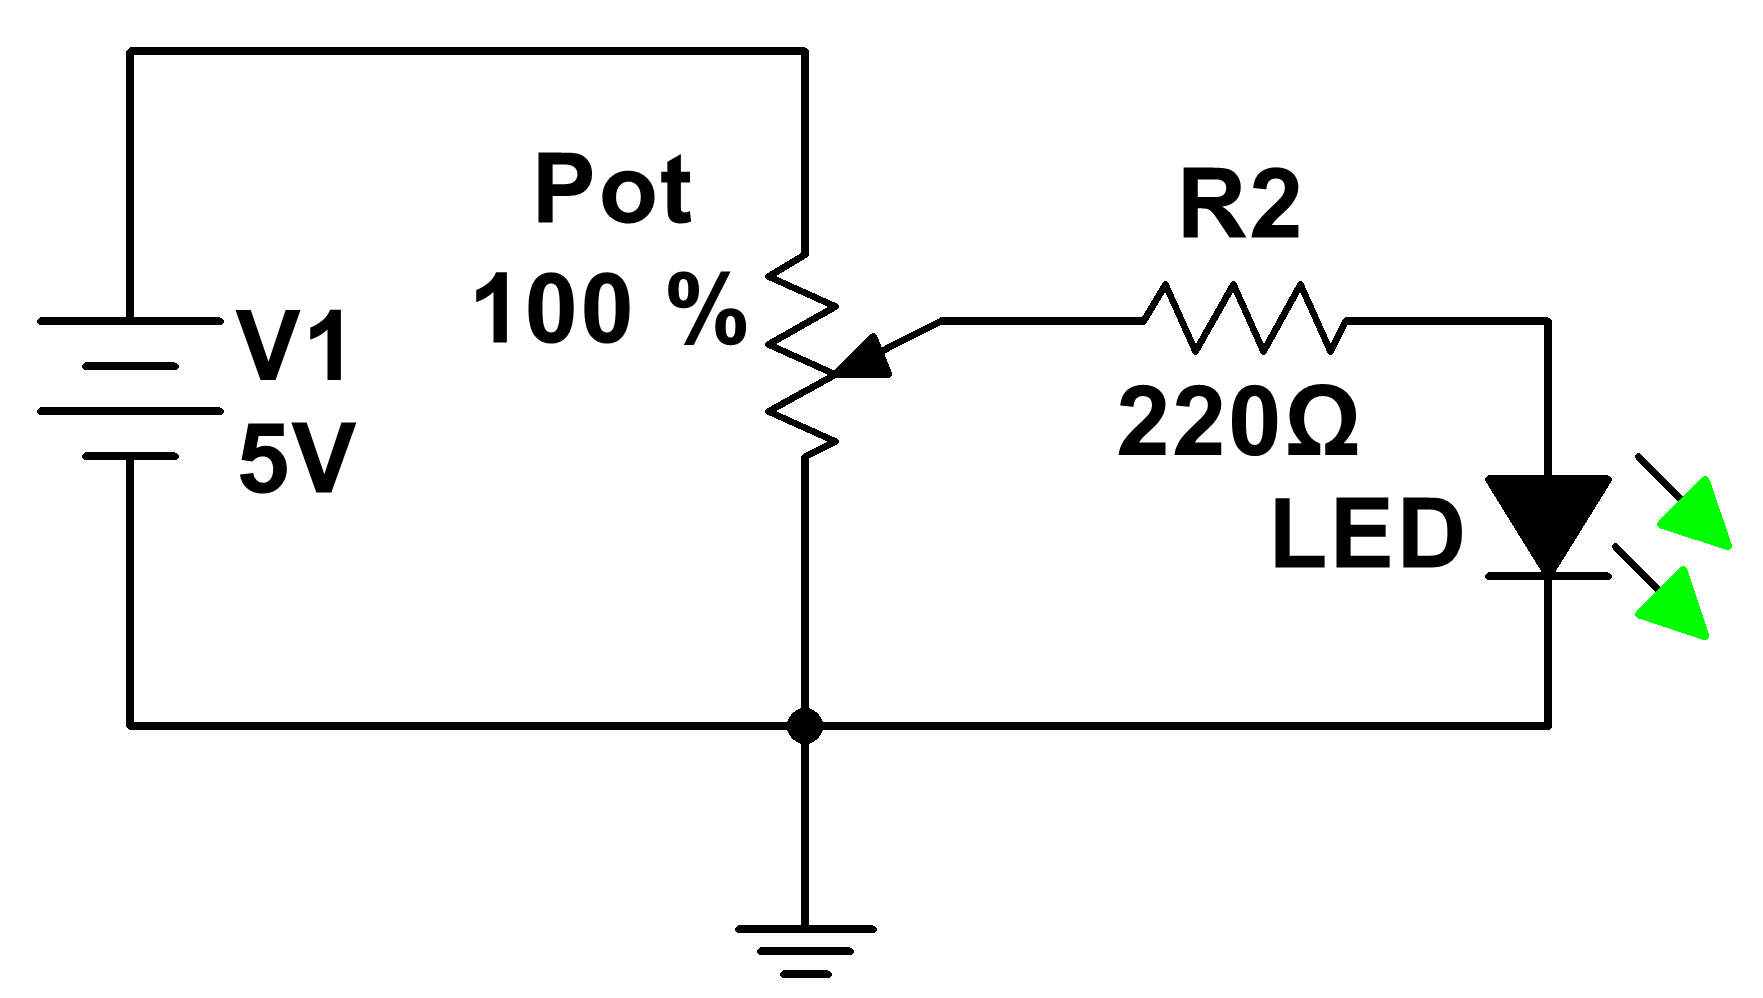
\includegraphics[width=6cm]{photos/lab/ledcircuit.PNG}
    \caption{Circuit schematic for experiment 3.1}
\end{figure}

\textbf{\underline{INSTRUCTIONS}}
\begin{enumerate}
    \item Build the circuit in \textit{Figure 3} above. You can use any color LED of your choosing. Leave the power supply off and ensure the voltage adjustment knob is set to 0.
    \item When the circuit is built, turn on the power to the DC power supply and adjust the voltage to 5V.
    \item Turn the potentiometer from fully counter clockwise to fully clockwise. Note the state of the LED (on, off) and the voltage drop across the LED when the potentiometer is turned fully clockwise and fully counterclockwise in the below table.
        \begin{table}[H]
        \centering
        \begin{tabular}{|l||l|l|l|} %c means centered left left alighned. Add more | for more lines between columns and more letters for more columns.
            \hline
                 &  Fully CCW & Fully CW   \\ \hline \hline
                 State of LED &     &       \\ \hline
                 Voltage across LED &     &       \\ \hline
        \end{tabular}
        \caption{}
        \end{table}
    \item Now, find the point where the LED just turns on. Measure the voltage across and current through the LED. Record them here. $V_{TO} = $ \underline{\hspace{2cm}} $I_{TO} = $ \underline{\hspace{2cm}}
    \item Note the state of the potentiometer at this turn on point. Find the resistance between pins 1 and 2. Find the voltage between pin 2 and ground. Record them here. $R_{12} = $ \underline{\hspace{2cm}} $V_{2} = $ \underline{\hspace{2cm}}
    
\end{enumerate}

\textbf{\underline{QUESTIONS}}
\begin{enumerate}
    \item Explain what is happening when you vary the potentiometer from fully counter clockwise to fully clockwise. What is happening to the LED? Why? Relate the behavior to the circuits topology using ohms law.
        \fillwithlines{1in}

    \item Compute the percentage that the potentiometer was turned away from the direction in \textit{Table 1} which corresponds to when the LED was off. Use the values from instruction 5.
    
        \framebox(439,100){}
        
    \item Explain why this computed percentage in the previous step is or is not expected. Relate this to how the potentiometer influences the delivery of the electricity to the LED.
        \fillwithlines{1in}
\end{enumerate}         

Now, continue with the same circuit, but replace the DC power supply and potentiometer with a waveform generator, such that the wave gen is applied accross an LED in series with a $220\Omega$ resistor. Leave the wave gen off.

\textbf{\underline{INSTRUCTIONS}}
\begin{enumerate}
    \item Turn the waveform generator on. Go to the channel setting by pressing the button \texttt{1} above the BNC connector and under the \texttt{Output Load} menu, enable \texttt{High Z}.
    \item Select the \texttt{Waveforms} button located right the display. Select the Sine wave and enter the \texttt{Parameters}. Use $f = 1 Hz$. Use a peak to peak amplitude of $V_{pp} = 5 - V_{TO} = $ \underline{\hspace{2cm}}. Use an offset of $V_{offset} = V_{TO} + \frac{V_{pp}}{2} = $ \underline{\hspace{2cm}}. Record the values in the space provided.
    \item Change the waveform from the sinusoid to a triangle wave. Use the same parameters as previously used and calculated. Observe the LEDs behavior.
    \item Change the waveform to a square wave. Use a peak to peak amplitude of $V_{pp} = 5V$. Use an offset of $V_{offset} = 2.5 V$. Use a frequency of $f = 1 Hz$. Observe the LEDs behavior.
    \item Increase the frequency of the square wave until the LEDs flashing becomes unnoticeable and it appears the LED is constantly illuminated. Record the frequency here. $f = $ \underline{\hspace{2cm}} Hz.
    \item Decrease the duty cycle of the square wave until the flashing becomes noticeable again. Record the value here. $Duty Cycle = $ \underline{\hspace{2cm}} \%
\end{enumerate}

\textbf{\underline{QUESTIONS}}
\begin{enumerate}
    \item Compare the behavior of the AC signals applied to the LED to that of with the potentiometer. How are they similar? How are they different?
        \fillwithlines{0.8in}
    \item Compare the behavior of the sine, triangle, and square waves. Compare each with the others. How are they similar? How are they different?
        \fillwithlines{1.25in}
    \item Compute the average voltage drop across by the LED with the square wave with duty cycle from instruction 6.
    
        \framebox(439,100){}    
    \item Compare the power consumption of the LED using the square wave from the previous question to that of a LED with a DC voltage of that of the square waves peak amplitude. What can be said about using the square wave as opposed to DC?
        \fillwithlines{1in}
    \item If the frequency were increased, what would happen? What would happen if the amplitude and offset were changed?
        \fillwithlines{1in}
\end{enumerate}

\checkoffsubsub %create a checkoff sub sub section. Details in style file.

\subsection{Controlling a DC motors speed and direction}

As seen in the previous experiment, the square wave is very powerful due to its ability to vary the amount of power delivered to a device by varying its duty cycle. In LEDs, this can adjust the amount of "on" time in a single period, effectively making the LED capable of appearing as always on but delivering less power. In the case of a DC motor, this variation of delivered power through the duty cycle changes the speed. Through the use of a DC motor controller, the PWM signal as well as signals that indicated the desired operation direction can be utilized to supply power from an alternative source. This is important in robotics controls as the microcontrollers output cannot supply enough power to operate the motors directly. Thus, an external IC the TB6612FNG motor driver can be utilized to operate the motors of a robot.

\begin{figure}[H]
    \centering
    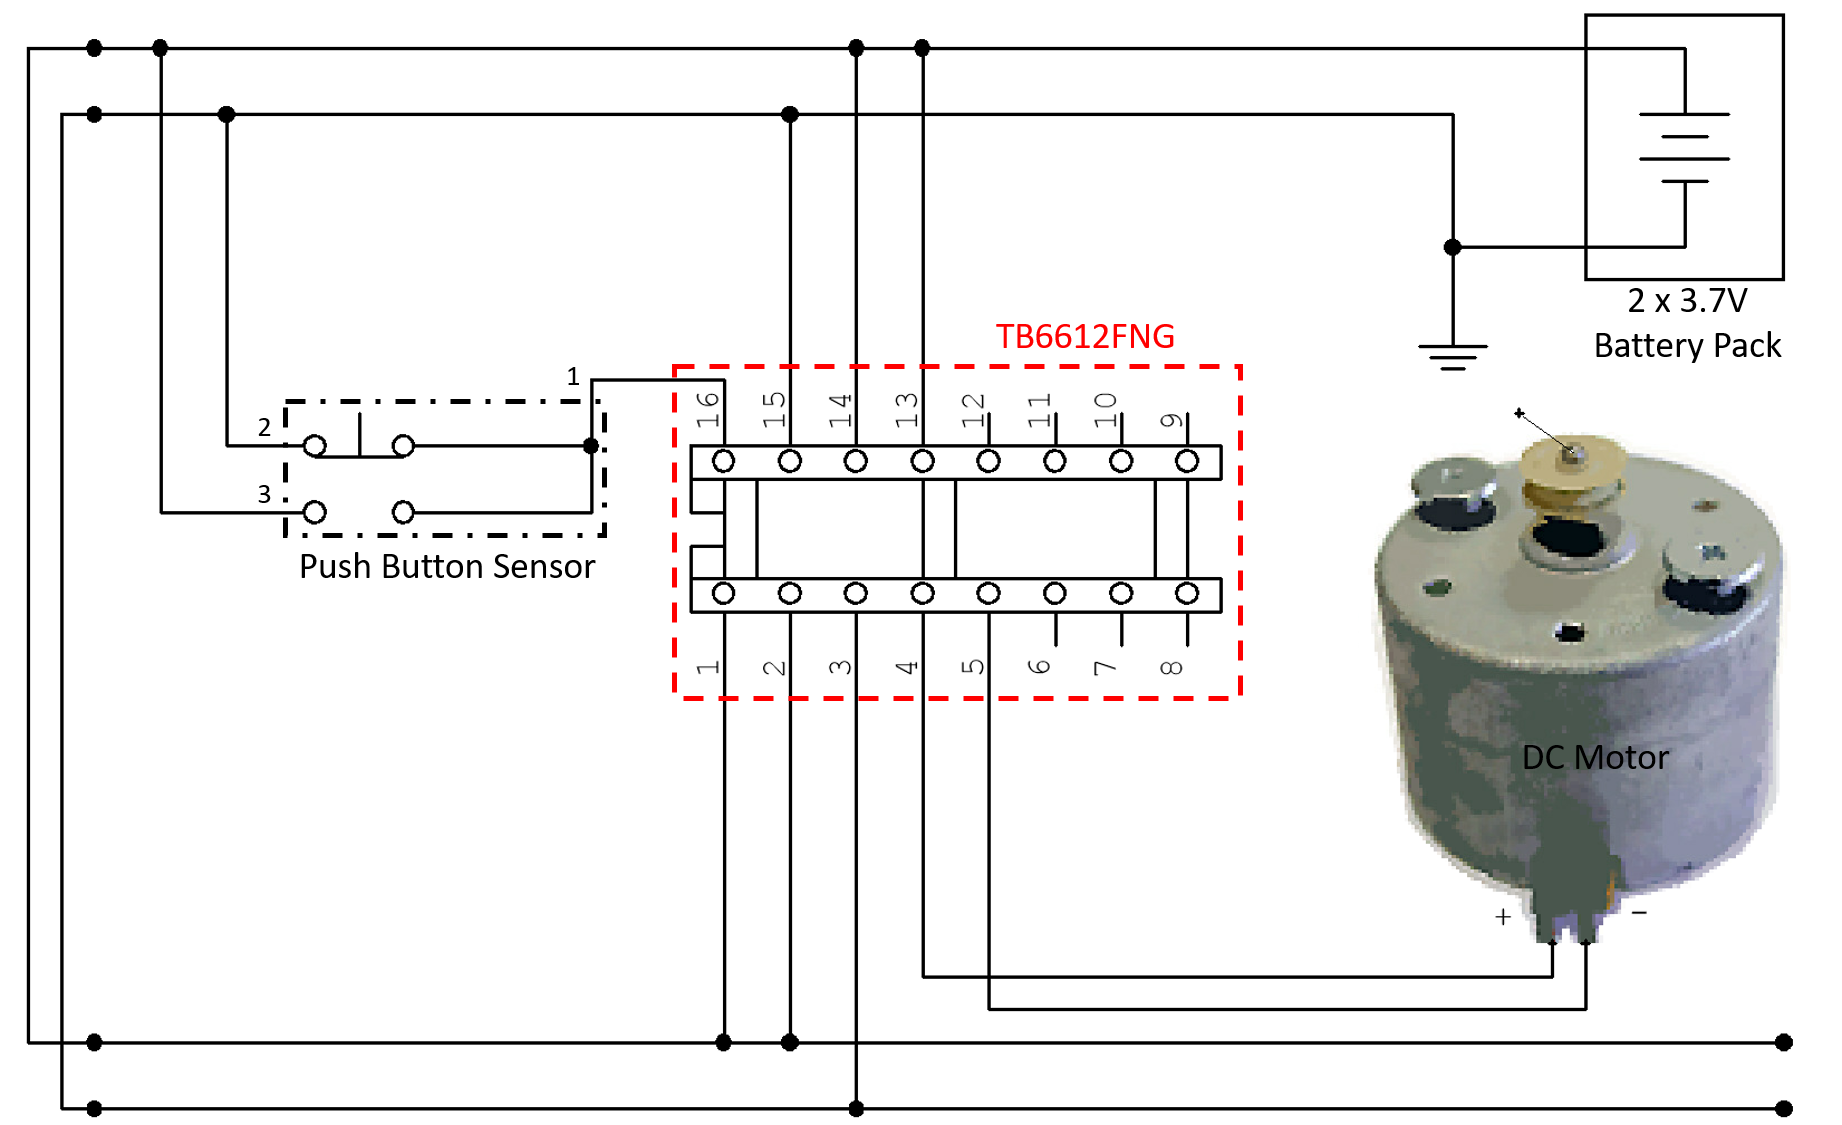
\includegraphics[width=12cm]{photos/lab/motorcircuitlabeled.png}
    \caption{Circuit schematic for experiment 3.2}
\end{figure}

\textbf{\underline{INSTRUCTIONS}}
\begin{enumerate}
    \item Collect the batteries from the battery charger and place them into the battery case. Make sure the switch on the case is in the off position.
    \item Build the circuit as shown in the schematic in \textit{Figure 4}. Do not turn the power switch on the battery case on. Note the two lines of wire at the top and bottom of the schematic resemble the power rails on your breadboard.
    \item When you have finished constructing the circuit, call the instructor over to verify the construction. 
    \item When the instructor has verified the circuit is built correctly, turn on the power switch to the batteries. 
    \item Press and hold the push button. Note the direction the motor spins. Let go of the pushbutton. Press the push button on and off rapidly and note what happens.
    \item Now, change pin 15 of the TB6612FNG chip to the positive rail of the power supply and change pin 14 to the ground rail.
    \item Press and release the pushbutton several times. Note the direction that the motor spins. 
\end{enumerate}
\newpage

\textbf{\underline{QUESTIONS}}
\begin{enumerate}
    \item Relate the operation of manually pressing the push button in this circuit to the pulse width modulation signal. How are they similar? How are they different?
        \fillwithlines{1in}
    \item In instructions 5 and 7, the motor should have spun when the push button was pressed. Compare the two operations. Is this expected? Why or why not?
        \fillwithlines{1in}
    \item Viewing a micrcontroller as a device that can output desired voltage signals to a desired device, explain how the microcontroller can replace the push button and signals on pins 13, 14, 15, and 16 to "control" a motor.
        \fillwithlines{1in}
\end{enumerate}

\textbf{\underline{INSTRUCTIONS}}
\begin{enumerate}
    \item Replace the push button at pin 16 with a waveform generator and reset the connections to pins 14 and 15 to that of the schematic.
    \item Turn on the wave gen and select the \texttt{Waveforms} button. Select the \texttt{Square Wave}.
    \item Select the \texttt{Parameters} button and change the peak to peak amplitude to $5V_{pp}$ and change the offset to $2.5V$.
    \item Start with a frequency of 1 kHz and duty cycle of 50\%.
    \item To turn on and off the signal from the wave gen, press the \texttt{1} button located above the output BNC connector and select to enable from the menu.
    \item Change the duty cycle of the waveform from 50\% to 25\%. Note the differences in \textit{Table 2}.
    \item Change the frequency above and below 1kHz significantly. Test 3 different duty cycles and note the differences in \textit{Table 2}.
\end{enumerate}

\begin{table}[H]
\centering
\begin{tabular}{|c|c|c|} %c means centered left left alighned. Add more | for more lines between columns and more letters for more columns.
    \hline
         \hspace{1.5cm}Frequency\hspace{1.5cm} & \hspace{1.5cm}Duty Cycle\hspace{1.5cm} & \hspace{1cm} Noteable differences \hspace{1cm} \\ \hline \hline
         1 kHz &  50\%   &       \\ \hline
         1 kHz &  25\%   &       \\ \hline
         1 kHz &  75\%   &       \\ \hline
               &         &       \\ \hline
               &         &       \\ \hline
               &         &       \\ \hline
               &         &       \\ \hline
               &         &       \\ \hline
               &         &       \\ \hline
                    
        
\end{tabular}
\caption{}
\end{table}

\textbf{\underline{QUESTIONS}}
\begin{enumerate}
    \item Explain the differences in the speed of the motor when the duty cycle was varied within a single frequency. Why is this?
        \fillwithlines{1in}
    \item When the frequency was changed, what did you notice?
        \fillwithlines{1in}
    \item If pin 13 were connected to ground, what would happen to the motor?
        \fillwithlines{1in}
    \newpage
    \item Could a DC power supply have replaced a battery pack in this experiment? Why or why not? When would a battery pack be a better choice over a power supply?
        \fillwithlines{1in}
\end{enumerate}

\checkoffsubsub

\section{Submission}

When you have finished all of the experiments in \textit{Section 3}, and have received a check off signature with all of the questions answered, you can begin to clean your station. Make sure all cables are put away, all equipment is powered off, and all circuit elements are disposed of appropriately. When you are finished cleaning, turn the packet into the instructor. You are free to leave if time remains.

\end{document}